\section{Information Retrieval and Retrieval-Augmented Generation}
Information Retrieval (IR) is the science of searching for documents, information within documents, and metadata about documents. Traditionally, IR relied on exact keyword matching and statistical methods like TF-IDF or BM25. However, these methods often fail to capture semantic nuances, such as synonyms or the context in which a technical term is used \cite{Manning2008Introduction}. In the era of Edge AI, the ability to retrieve precise technical specifications from disparate sources—such as STM32 datasheets, user manuals, and community forums—is a prerequisite for automated model deployment.

\subsection{From Keyword Search to Semantic Retrieval}
The advent of deep learning transformed IR through the use of \textbf{Word and Document Embeddings}. By mapping text into a high-dimensional vector space where semantically similar concepts are clustered together, models can perform "semantic search." A query like "how to reduce RAM usage on STM32" can effectively retrieve documents discussing "memory optimization" or "flash-to-RAM mapping," even if the exact keywords do not overlap. Vector databases (e.g., Chroma, FAISS, Pinecone) are used to store these embeddings and perform efficient similarity searches using metrics like Cosine Similarity \cite{naveed2024comprehensiveoverviewlargelanguage}.

\subsection{Retrieval-Augmented Generation (RAG)}
While LLMs possess significant internal knowledge, they suffer from "knowledge cutoffs" (inability to access information post-training) and "hallucinations" (generating plausible but false data). \textit{Retrieval-Augmented Generation (RAG)} addresses these gaps by grounding the LLM's response in external, verified facts \cite{Gao2024RetrievalAugmentedGN}. 

As shown in Fig. \ref{fig:rag}, a standard RAG pipeline consists of three phases:
\begin{enumerate}
    \item \textbf{Retrieval:} Given a user query, the system retrieves relevant chunks of text from a knowledge base or via the web.
    \item \textbf{Augmentation:} The retrieved context is appended to the original prompt, providing the LLM with the necessary background information.
    \item \textbf{Generation:} The LLM generates a response based on both its internal weights and the provided external context.
\end{enumerate}

\begin{figure}[ht]
    \centering
    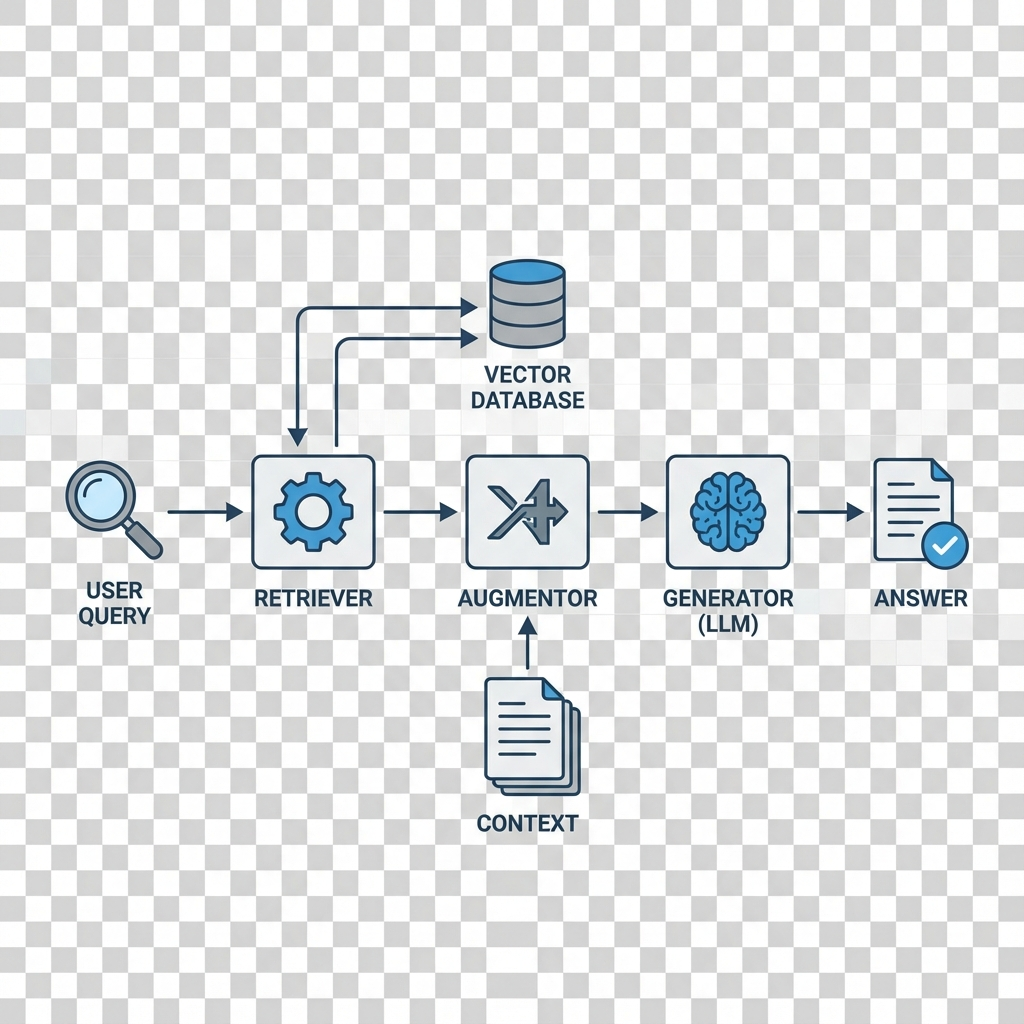
\includegraphics[width=1\textwidth]{chap2/figure/rag.png}
    \caption{Operation cycle of a Retrieval-Augmented Generation system \cite{medium_rag_workflow}.}
    \label{fig:rag}
\end{figure}

\subsection{Web Research and Hardware Knowledge Grounding}
In the developed framework, RAG is extended beyond static document sets. The "Web Research" branch utilizes live search APIs (e.g., Google Search, Tavily) to fetch the latest information on STM32 boards, STEdgeAI tool versions, and cutting-edge optimization libraries. This dynamic retrieval ensures that the agent's decisions—such as recommending an MCU for a specific neural network architecture—are based on up-to-date benchmarks and hardware compatibility lists rather than outdated training data.

\subsection{Limitations and Mitigation Strategies}
Despite its advantages, RAG inherits challenges related to retrieval quality and context management. "Retriever failure" occurs when the search engine fails to find relevant context, leading to grounded but irrelevant generation. "Generator failure" occurs when the LLM ignores the provided context or fails to resolve contradictions between its internal weights and the retrieved data \cite{Gao2024RetrievalAugmentedGN}. Advanced systems mitigate these through re-ranking (scoring retrieved chunks before generation) and self-correction loops, where the system evaluates its own output for faithfulness and relevancy.
